\documentclass{beamer}
\usepackage{beamerthemeshadow}
\usepackage{graphicx}
\usepackage{color}
\usepackage[utf8]{inputenc}
\usepackage{hyperref}
\usepackage[flushleft]{threeparttable}
\usepackage[english,serbian]{babel}
\definecolor{beamer@darkred}{rgb}{0.85,0.1,0.1}
\setbeamercolor{structure}{fg=beamer@darkred}

\title{Tehničko i naučno pisanje}
\subtitle{VAR tehnologija}
\author{Luka Šešelja, Ognjen Arsenijević, Ognjen Radivojević}
\institute{Matematički fakultet\\Univerzitet u Beogradu}
\date{\footnotesize{Beograd, 2022.}}

\begin{document}
\begin{frame}
\titlepage
\end{frame}

\begin{frame}[fragile]{Literatura}
    \begin{itemize}
        \item 
    \end{itemize}
\end{frame}

\begin{frame}
  \frametitle{Pregled}
  \tableofcontents
\end{frame}

\section{Uvod}

\begin{frame}
  \frametitle{VAR tehnologija}
  \begin{itemize}
    \item Šta je VAR tehnologija?
    \item Prednosti VAR-a
    \item Kontroverznost VAR-a
  \end{itemize}
\end{frame}

\begin{frame}
  \frametitle{Istorija}
  \begin{itemize}
    \item Prva ideja o upotrebi video tehnologije u fudbalu
    \item Prvi test uživo
    \item Monitor pored terena
    \item Zvanična implementacija VAR-a u pravila fudbala
    \item VAR danas
  \end{itemize}
\end{frame}

\section{Primena VAR tehnlogije u praksi}

\begin{frame}
  \frametitle{Slucajevi u kojima se koristi VAR tehnologija}
  \begin{itemize}
    \item Gola ili prekršaja koji dovodi do gola.
    \item Penala ili prekršaja koji dovodi do penala.
    \item Dodele direktnog crvenog kartona.
    \item Greške pri identifikovanju igrača.
  \end{itemize}
\end{frame}

\begin{frame}
  \frametitle{Podešavanje kamera}
    \begin{figure}[h!]
    \begin{center}
    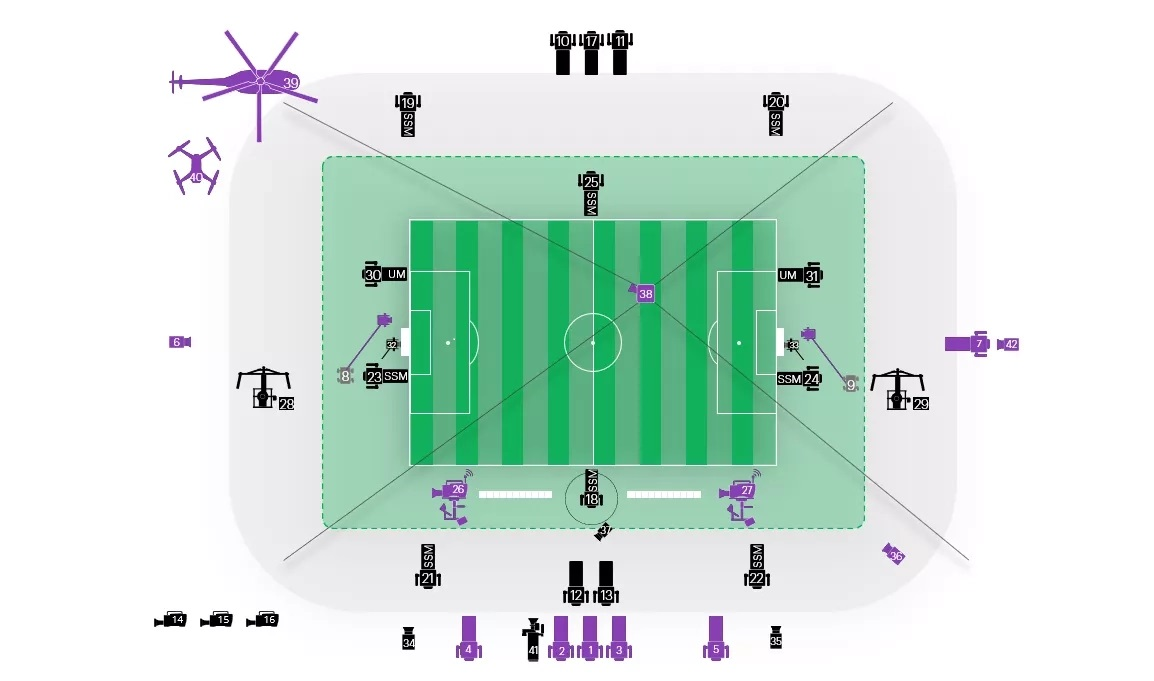
\includegraphics[scale=0.30]{Var sistem.jpeg}
    \end{center}
    \caption{Raspored kamera na terenu u okviru VAR sistema}
    \label{fig:kamere}
\end{figure}
\end{frame}
\begin{frame}
  \frametitle{VAR tim}
    \begin{figure}[h!]
    \begin{center}
    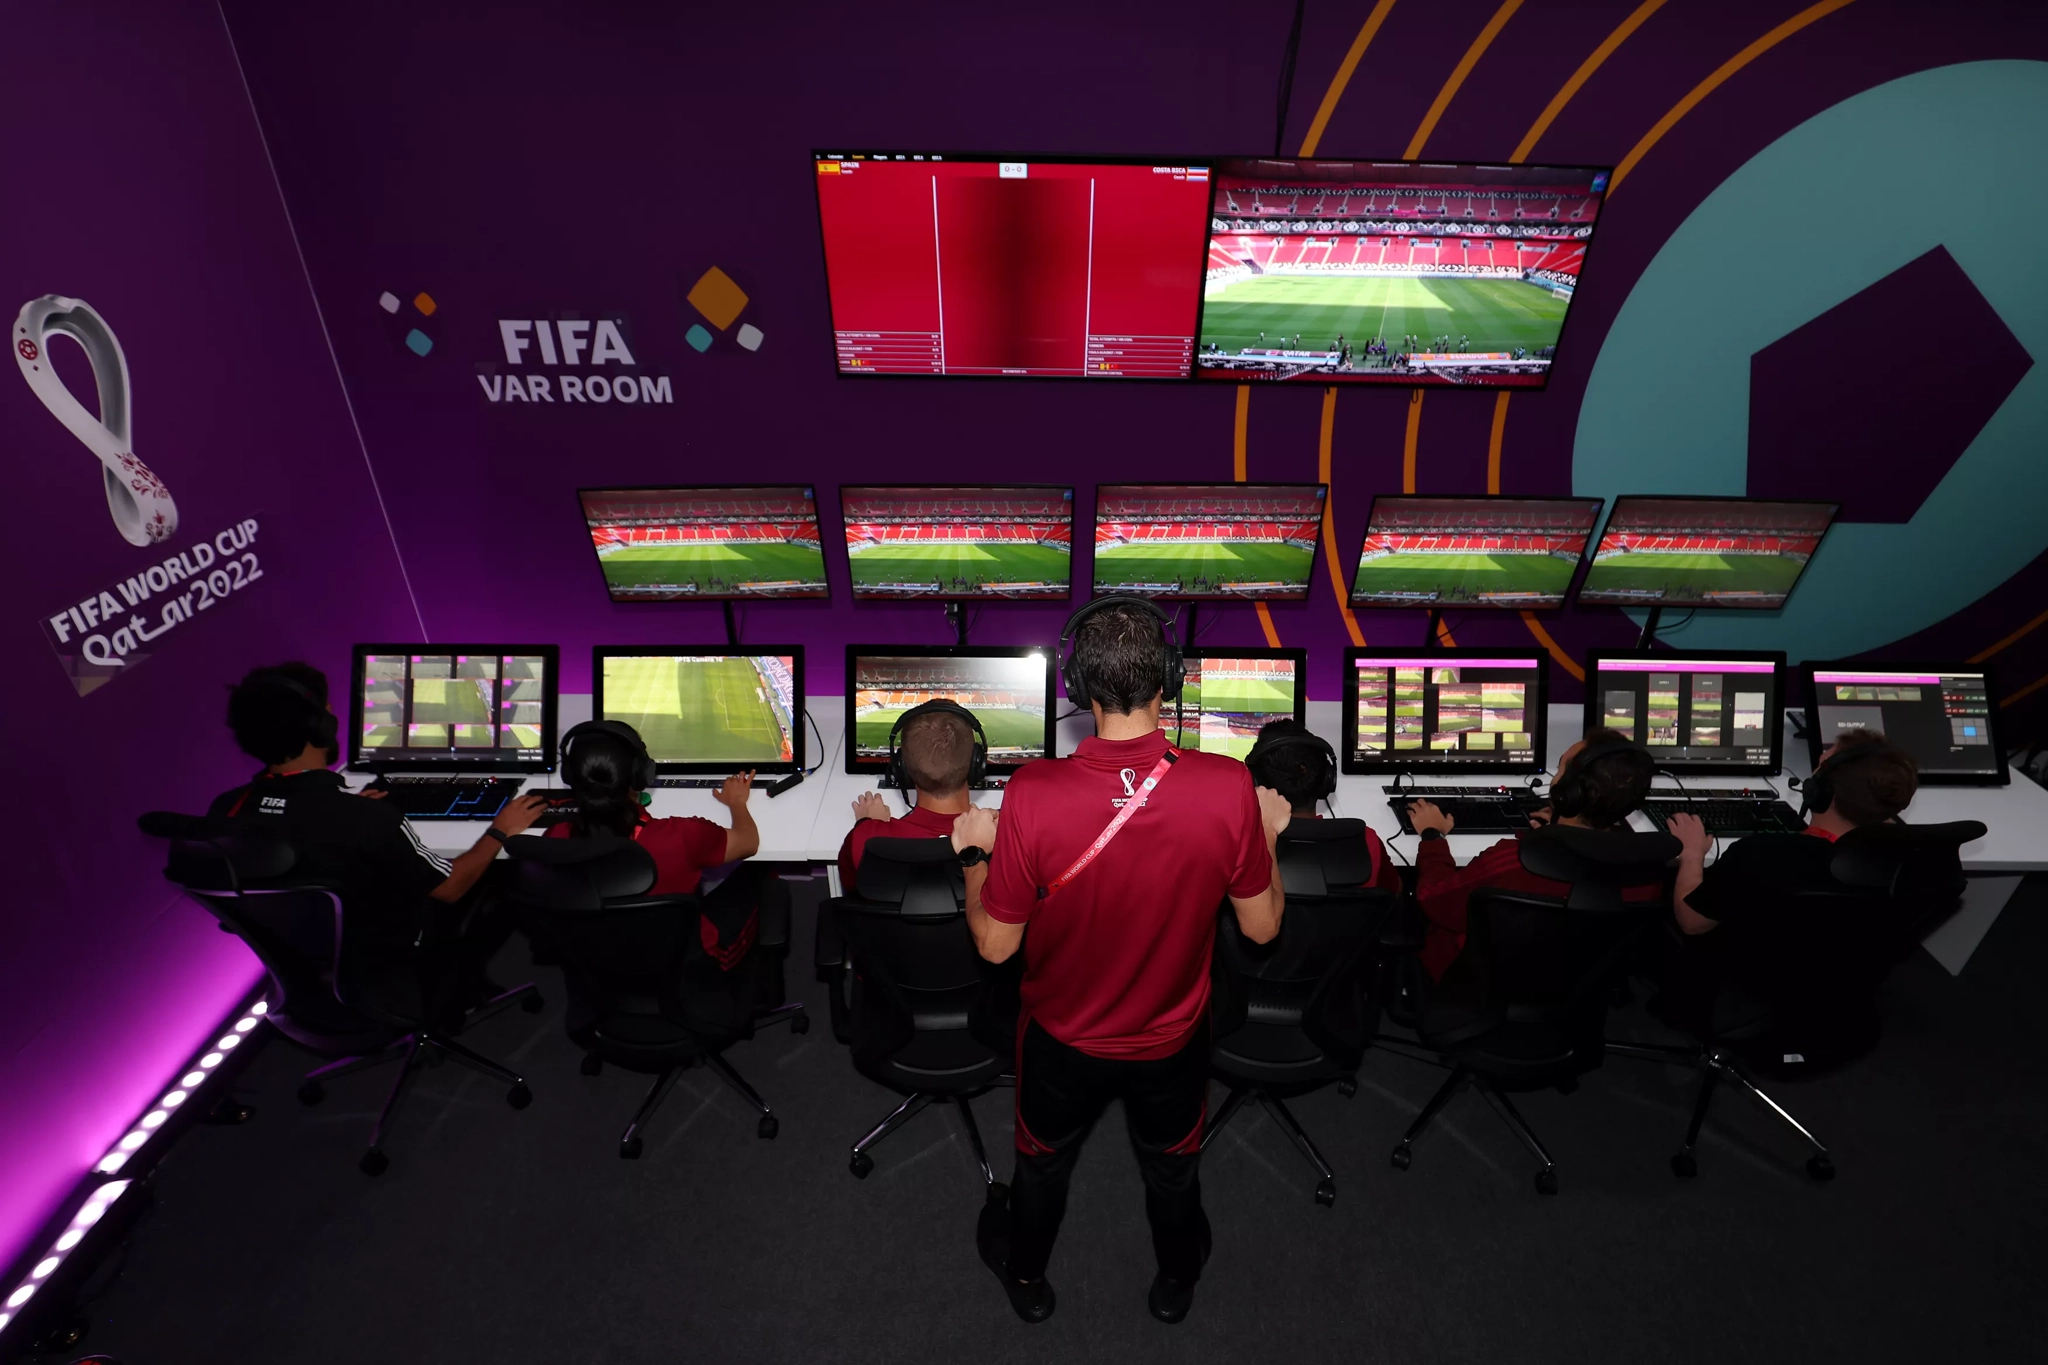
\includegraphics[scale=0.20]{var.png}
    \end{center}
    \caption{Članovi VAR tima}
    \label{fig:vartim}
\end{figure}
\end{frame}

\section{Preciznost provera}

\begin{frame}
  \frametitle{Preciznost i trajanje provera}
  \begin{itemize}
    \item  Ispravnost sudijske odluke
    \item  Trajanje provere i pregleda
    \item  Statistička analiza
  \end{itemize}
\end{frame}

\begin{frame}
  \frametitle{Preciznost odluka (\%)}
  \begin{itemize}
    \item  Tačnost i broj provera
    \item  Siva zona i sudijske odluke
    \item  Tipovi indidenata
  \end{itemize}
\end{frame}

\section{Zaključak}

\begin{frame}
  \frametitle{Zaključak}
  \begin{itemize}
    \item  Skinut pritisak sa sudija na terenu
    \item  Šta je VAR doneo dobro
    \item  Šta je VAR doneo loše
  \end{itemize}
\end{frame}


\end{document}
